\subsection*{b)}

\section*{Antwort}

Es empfiehlt sich, eine \textbf{Aggregationsbeziehung} (\cite[48]{Bal05}) zu modellieren: Abbildung~\ref{fig:aufgabe-4-teil-b} zeigt einen Entwurf für eine Umsetzung in Java.\\

\begin{figure}
    \centering
    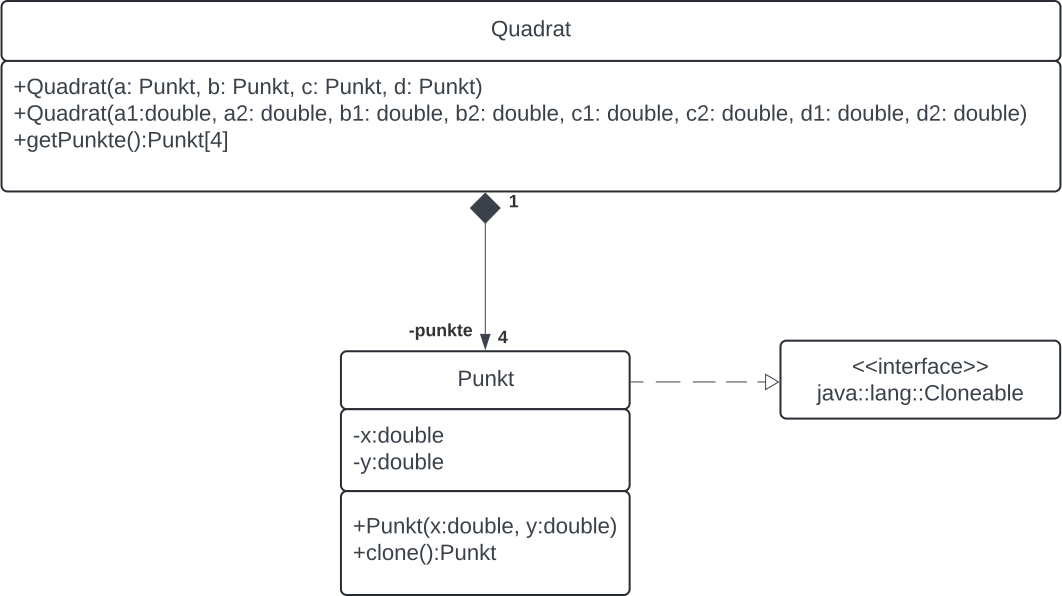
\includegraphics[scale=0.5]{chapters/aufgabe 4/img/aufgabe4b}
    \caption{Modellierung der Klassen \textit{Quadrat} und \textit{Punkt} und ihrer Aggregationsbeziehung.
    Ein \textit{Quadrat} besteht immer aus $4$ Objekten des Typs \textit{Punkt}. Ein Objekt vom Typ \textit{Punkt} kann zu keinem oder bis zu 3 Objekten des Typs \textit{Quadrat} gehören. Eine Navigierbarkeit geben wir nicht explizit an, da ein Ganzes implizit weiß, aus welchen Teilen es besteht. Die andere Richtung lassen wir undefiniert, da nicht klar hervorgeht, ob ein Punkt auch über seine Zugehörigkeit zu einem Quadrat wissen muss (Quelle: eigene)}
    \label{fig:aufgabe-4-teil-b}
\end{figure}

\noindent
Wie auf der Skizze ersichtlich, kann ein Objekt vom Typ \code{Punkt} ohne Beziehung zu einem Objekt vom Typ \code{Quadrat} existieren.\\
Des Weiteren kann ein Punkt zu max. $3$ Quadraten gehören.\\
Eine  \textbf{Aggregationsbeziehung} stellt sicher, dass der Entwurf diese Anforderung ausdrückt.\\

\subsection*{Anmerkung}
In der Analyse kann diskutiert werden, ob ein Punkt auch zu max. $4$ Quadraten als ``Mittelpunkt`` gehören kann.\\
Außerdem wäre zu klären, ob \code{Punkt} als \textbf{Immutable}\footnote{
    vgl. \cite[21]{LG00}; eine mögliche Implementierung geometrischer Figuren wird ebenda auf S. 94 f. angerissen
} implementiert werden soll, sofern sich die Änderungen eines Punktes \textit{nicht} auf alle assoziierten Aggregatobjekte auswirken soll\footnote{
    s. a. \textbf{Aliasing-Bugs}, \url{https://martinfowler.com/bliki/AliasingBug.html}, abgerufen 18.05.2024
}.


